\section{Bannerová reklama}
    \begin{quote}
        \enquote{\emph{Cílem bannerové reklamy je nejen zprostředkovat reklamní sdělení, ale i zabezpečit, aby se recipient velmi jednoduchou aktivitou
        (kliknutím na banner) přesunul na požadovanou webovou lokalitu (firemní stránku, stránku značky, stránky produktu/značky na sociální síti atd.).}}
        (SVĚTLÍK, J., 2017) \cite{svetlik:reklama}
    \end{quote}

    V této části se práce více zaměřuje na bannerovou reklamu.
    Teorie a efektivita tohoto typu inzerce je zde rozebrána jako první a více do detailu. \cite{banner:advertising}

    \subsection{Formáty zobrazení}
    První webový banner se objevil na internetu v roce 1994. V té době se bannery objevovali nejčastěji jako statický obrázek ve formátu
    JPEG nebo PNG. Tento způsob zobrazení se udržel dodnes. Dynamický obsah v podobě animace bylo schopný zobrazit formát GIF a to v podobně pohyblivých obrázků.
    Společnost Macromedia s jejich technologií \emph{Flash} dokázali do bannerů přidat i možnosti interakce v podobě animací nebo přehrání zvuku při
    pohybu kurzoru myši nad bannerem. Dnes už technologie Flash z důvodu bezpečnosti a HW nároků není ve významných internetových prohlížečích podporována a
    dá se plně nahradit spojením HTML a JS kódu. 

    \subsection{Statický nebo dynamický banner}
    Statický banner je pouhým obrázkem, který se nijak nehýbe a nemá možnost interakce s uživatelem. S nástupem bannerů na Internet se u
    spotřebitelů začal objevovat fenomén zvaný \emph{bannerová slepota}. Bylo zjištěno, že někteří uživatelé podvědomě bannery na standardních místech
    úplně ignorují a nevnímají je. Proti tomuto jevu dokáži efektivně bojovat dynamické bannery.
    I krátká animace dokáže zachytit pozornost oka a tím lépe působit na cílové publikum.
    Toto se dá jednoduše změřit při porovnání CTR statických a dynamických bannerů.

    \subsection{Rozměry bannerů}
    Některé ze standardních rozměrů bannerů (v px) a jejich názvy lze vidět na obrázku \ref{fig:banner-sizes}. Podle rozlohy se zobrazují na jiných částech webových stránek nebo
    mobilních aplikací. S rozměry se také pojí velikost souborů. Reklamní sítě mívají na nahrané bannery limity velikostí.
    Čím menší velikost, tím rychleji se dokáže banner načíst. Nejčastější limit bývá 150~KB. Toto je více rozebráno v kapitole o reklamních sítích.

    \begin{figure}[h]
        \centering
        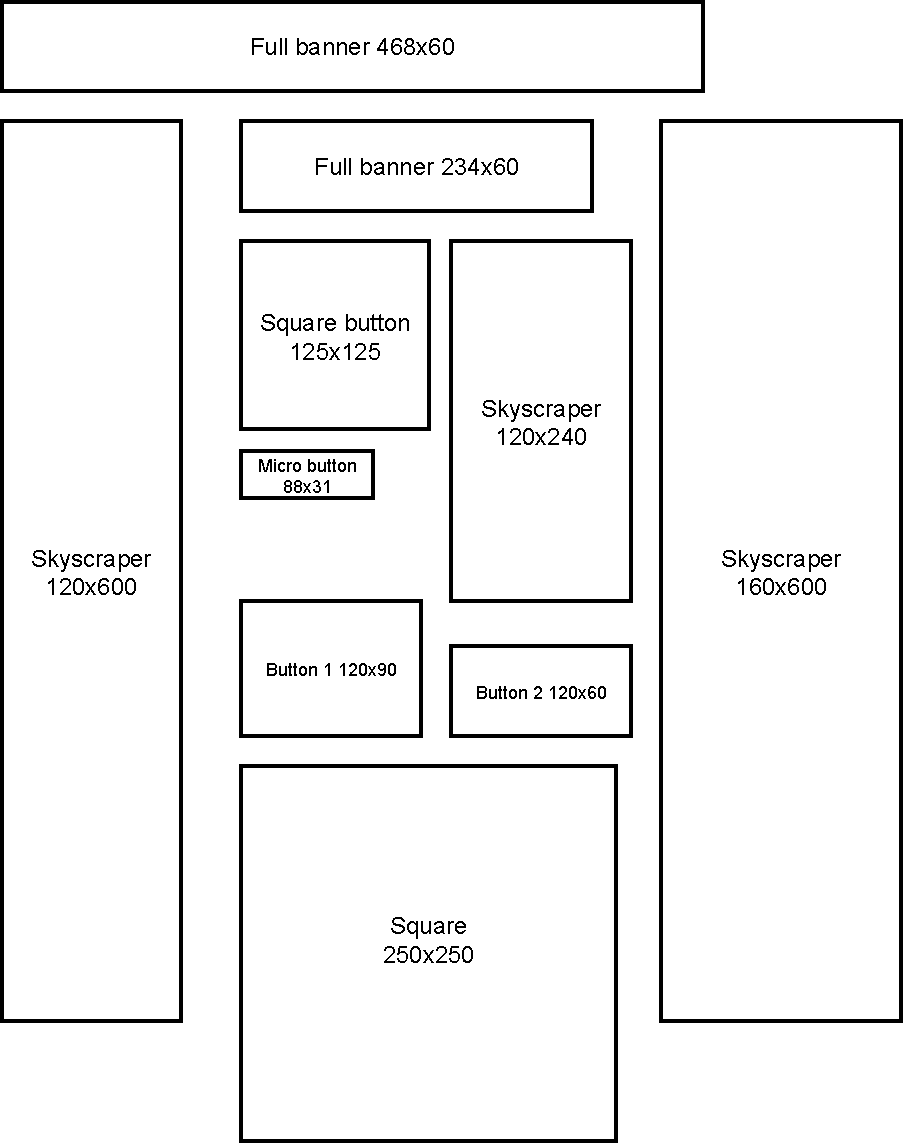
\includegraphics[width=1\textwidth]{Figures/banner-sizes.pdf}
        \caption[Velikosti bannerů]{Standardní používané velikosti bannerů}
        \label{fig:banner-sizes}
    \end{figure}

    \subsection{Jak vytvořit dobrý banner}
    Jak měřit efektivitu reklamy se zmiňuje část \ref{ssec:online-ad-metrics}. Tato část se věnuje tomu, jak banner vytvořit,
    aby již zpočátku co nejvíce upoutal zákazníky. \cite{banner:design}
    Reklamní banner se skládá ze 4 základních částí. Těmi jsou:
    \begin{itemize}
    \item logo inzerenta,
    \item titulek (komerční sdělení),
    \item pozadí,
    \item výzva k akci (CTA).
    \end{itemize}
    Na banneru se může nacházet více prvků, je však důležité, aby tyto hlavní části splnily doporučená pravidla, která jsou zde postupně rozebrána.

    \subsubsection{Logo}
    Pokud je to možné, mít logo na banneru je velice důležité. Pomáhá budovat povědomí o značce a napovídá zákazníkovi na čí webovou stránku by se měl dostat.
    Mělo by být dobře viditelné, ale nemělo by opticky přebíjet titulek nebo výzvu k akci.

    \subsubsection{Pozadí}
    Co se pozadí týče, na výběr jsou 2 varianty. Buď celobarevné nebo fotografie. Obojí má svá pro i proti. Pokud se banner snaží prodat nějaký produkt,
    je vhodnější vynechat obrázkové pozadí. Jednobarevná pozadí vytváří přirozený kontrast s výzvou k akci.
    Produkt na ni dobře vynikne a neodvádí pozornost od titulku. Naproti tomu, pokud se vytváří reklama na určitou službu nebo
    produkt nefyzického charakteru (nejčastěji software, IT služby) lze fotografií na pozadí ilustrovat onu nabízenou věc. 

    \subsubsection{Titulek}
    Doporučuje se spíše krátký text. Za úkol má přilákat pozornost možného zákazníka, tím pádem rozměrově zabírá větší část banneru.
    Podstatné kritérium je, aby byl text opět dobře čitelný. Proto je zapotřebí zvolit kontrastní barvu textu s dobře čitelným fontem.
    Řez písma by neměl být příliš tenký, jinak by text mohl splývat s pozadím nebo se špatně číst. Efekty typu zkosení se moc nedoporučují a
    někteří poskytovatelé reklamních sítí je vůbec nepovolují. 

    \subsubsection{Výzva k akci}
    Měla by u diváka vyvolat pocit nutnosti na banner kliknout. Zároveň by měla být dobře viditelná hned po titulku.
    Proto se často vyskytuje v podobě tlačítka s vhodně zvolenou barevnou kombinací.
    Umístění blíže k titulku diváka přirozeně navede.


\endinput